\section{Calendar}

The calendar is a new feature in SalesPoint 2011 to manage appointments. 

\begin{figure}[ht]
	\centering
  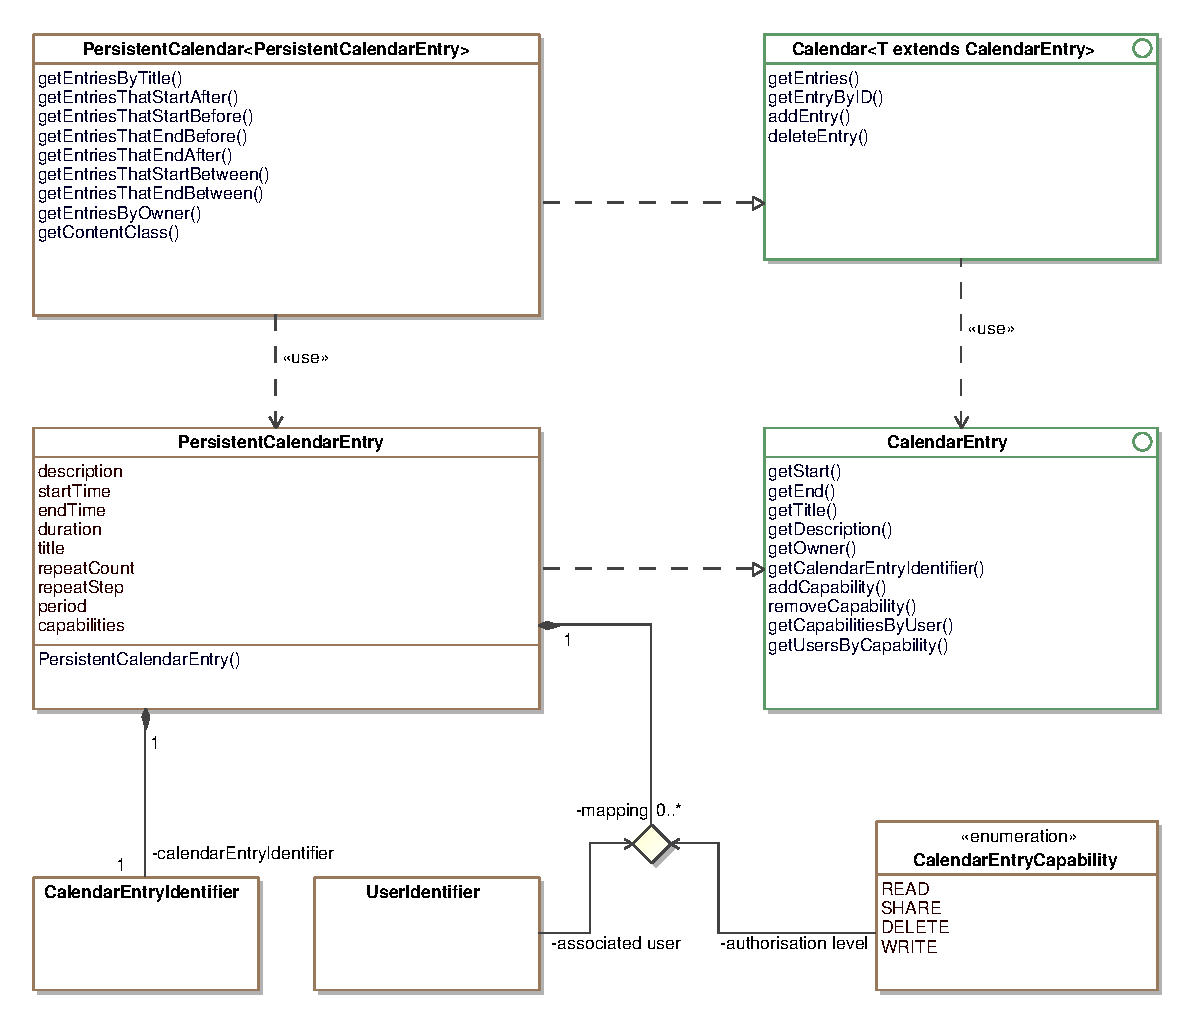
\includegraphics[width=1.0\textwidth]{images/Calendar_Overview.eps}
	\label{calendar_overview}
	\caption{Calendar - Class Overview}
\end{figure}

\subsection{\code{Calendar} - The central menagement for appointments}
The calendar is an interface that provides simple functionality to store calendar entries persistently in and recover them from the underlaying database.
With the \code{PersistentCalendar}-class there exists an implementation of the calendar interface that can be worked with. This class provides methods
to add and remove entries and filter them by different criterias.
There are some predefined methods for useful filters but also one that takes a user defined filter. The predefined filters are queries with predicates to select the right entries. When a user defined filter is used, all entries will be selected and the filter will be invoked for every entry.  
The \code{PersistentCalendar} calendar itself has no identifier or other attributes, it's just a container that provides methods to easy manage all calendar entries.
So there is no need to keep a reference to any calendar object, every time one is needed, it can be created new.


\subsection{\code{CalendarEntry} - Keeps information about a single appointment}

With \code{CalendarEntry} there exists an interface to set, store and access information about a single appointment, which is implemented
by \code{PersistentCalendarEntry}.
Every \code{PersistentCalendarEntry} must have an owner, title, start and end date.
Typically the owner is the creator of the entry and also gets all capabilities for this entry.
Capabilities are
\begin{itemize}
    \item \code{READ} - indicates who can read this entry
    \item \code{WRITE} - indicates who can change this entry
    \item \code{DELETE} - indicates who can delete the entry
    \item \code{SHARE} - indicates who can share the entry to other users
\end{itemize}.
All of these capabilities, can be given to and removed from a user in relation to this specific entry.
Because a calendar entry does not check if a user has the capability to do something with it, the programmer has to check the capabilities before manipulating the entry.
Besides the minimum information a calendar entry can also have a description which provides more information about it and a repeat count and repeat step which say how 
often the entry will be repeated and how long the timespan between two repetitions is.
There are some conditions for the time specific attributes of an calendar entry: First, the start must not be after the end. So a appointment can have a timespan if the end is after the start or it can be a single point in time, like a deadline or something like this, if start and end are equal.
Second, the repeat step, which is the time between two repetitions must be greater than the duration of the entry, so an entry does not overlap with the next repetition of itself.
Third, if repeat count is zero, the repeat step will not be attended, if repeat count is greater zero or -1, what means endless repetetion, the repeat step will be checked to follow the second point.
All attributes of the entry can be changed, except of the owner, who will be defined when the entry is created and then becomes immutable. 